\label {fs-discussion}

In this section, we discuss and demonstrate the main pitfalls which arise with the data flow. The purpose of our evaluation is to investigate the applicability of stream processing systems as a {\em tool} for building text classification pipelines rather than to compare various machine learning models. We concentrate on a question on how distributed stream processing features may affect reproducibility and reliability of classification results.

For experiments, we used an implementation of the proposed data flow on top of Apache Flink~\cite{Carbone:2017:SMA:3137765.3137777}. Apache Flink is a state-of-the-art industrial stream processing engine that is one of the most performant among competitors~\cite{karimov2018benchmarking, S7530084}. The experiments were performed on a single 4 core CPU 8GB RAM machine with 2 Flink workers. Such setting is chosen to show that issues can be faced even in a deployment with a limited asynchrony. As a dataset, we used an open corpus of news articles from Russian media resource lenta.ru~\cite{lentaru}. This dataset contains documents, which are labeled by one of 90 different topics such as {\em sport}, {\em politics}, {\em science}, etc. For the experiments, we generated a stream consisting of articles from the dataset. Processing {\em latency} in such setting is a time period between article arrives at the system entry and a corresponding label given by a classifier is released. 

We used multinomial logistic regression model as a classifier. We mainly considered the multi-classification problem, but also observed the label probability distribution obtained by an article. For instance, text about novel research in sports food may be denoted as 70\% about sport, 20\% about science and 10\% about food. In this case, it may be reasonable to take into consideration the top $n$ most probable labels rather than only the winner topic (sport).

\subsection{Reproducibility}

Users of popular open-source machine learning libraries like sklearn~\cite{sklearn_api} are used to obtain results which are unbiased by an execution environment. Migration to batch processing systems like Hadoop~\cite{hadoop2009hadoop} or Spark~\cite{Zaharia:2016:ASU:3013530.2934664} usually do not cause any significant issues, because these engines mostly hide effects of asynchronous processing from a user and provide deterministic results. On the contrary, most distributed stream processing engines are non-deterministic due to processing model aiming to low latency. Therefore, the main challenge regarding reproducibility of streaming machine learning pipelines is to achieve predictable results, while keeping low processing latency.

\subsubsection{Races in the data flow}
The issue is that there is a race between documents in the data flow before IDF update. Hence, IDF features of the words in articles may vary from run to run. For example, let us consider two documents stream: the first one contains word {\em cat}, while the second consists of {\em cat} and {\em dog}. If the first document is processed before the second, IDF for the word {\em cat} within TF-IDF features of the second document will be 1, while otherwise, it will be 0.

To show how this behavior affects text classification results we made 10 runs on a stream consisted of 10 000 news articles. We compared the most probable 1,2,3,4,5 obtained labels for the same documents between runs. Our comparison was order-sensitive: if top 2 labels for the document on the first run is [sport (50\%), science (20\%)], but on the second run [science (50\%), sport (20\%)], then we denoted these results as varied. 

Table~\ref{race_table} demonstrates the results of the experiment. Most probable labels were assigned differently for 56 out of 10 000 articles. With the growth of the number of the labels that we consider, the percent of varied results significantly increases: 1270 articles achieved different top 5 labels on the average. These results indicate that the issue may influence the classification results and makes them hardly reproducible between independent runs. Another negative effect of non-deterministic data flow is an increase in results variance. It may be unclear which reason causes accuracy changes: modification of the model or just another order of IDF updates.

\begin{table}[htbp]
\caption{Effects of races in the data flow}
\begin{threeparttable}
\begin{tabular}{lcl}
Top labels for comparison    & \% of varied results & std    \\
\hline
1   &   0.56    &   0.06    \\
2   &   2.38    &   0.14    \\
3   &   5.27    &   0.22    \\
4   &   9.27    &   0.35    \\
5   &   13.7    &   0.53    \\
\end{tabular}
\end{threeparttable}
\label{race_table}
\end{table}

\subsubsection{Overhead on enforcing reproducibility}

A straightforward technique to avoid races before IDF update is to define a synthetic total order on input documents and to enforce such order before the operation that modifies IDF. In Flink, the order can be defined using timestamps assigned to input elements. Order enforcement is implemented using custom {\it ProcessFunction} that buffers all words before IDF update. In order to flush this buffer, there is a need to ensure that all words from the document with a particular timestamp have arrived. Such guarantee can be provided by {\em low watermarks} mechanism. Low watermarks are service stream elements which go through the same network channels as ordinary elements and guarantee that there are no items with a given or less timestamp up to the stream. Hence, we can flush parts of the buffer when a corresponding watermark arrives. Such implementation follows an {\em out-of-order} processing approach~\cite{Li:2008:OPN:1453856.1453890}.

Figure~\ref{reproducibility} demonstrates the comparison in latency between reproducible and irreproducible data flows. We compare $50^{th}$, $75^{th}$, $95^{th}$, and $99^{th}$ percentile of distributions, which clearly represent the performance from the perspective of the users' experience. Latency overhead is 50\% (11 ms) for the median and 24\% (28 ms) for the 99th percentile. This behavior indicates that the overhead is moderate in a general case. However, it may be sensitive for applications with extremely low latency requirements.

\begin{figure}[htbp]
  \centering
  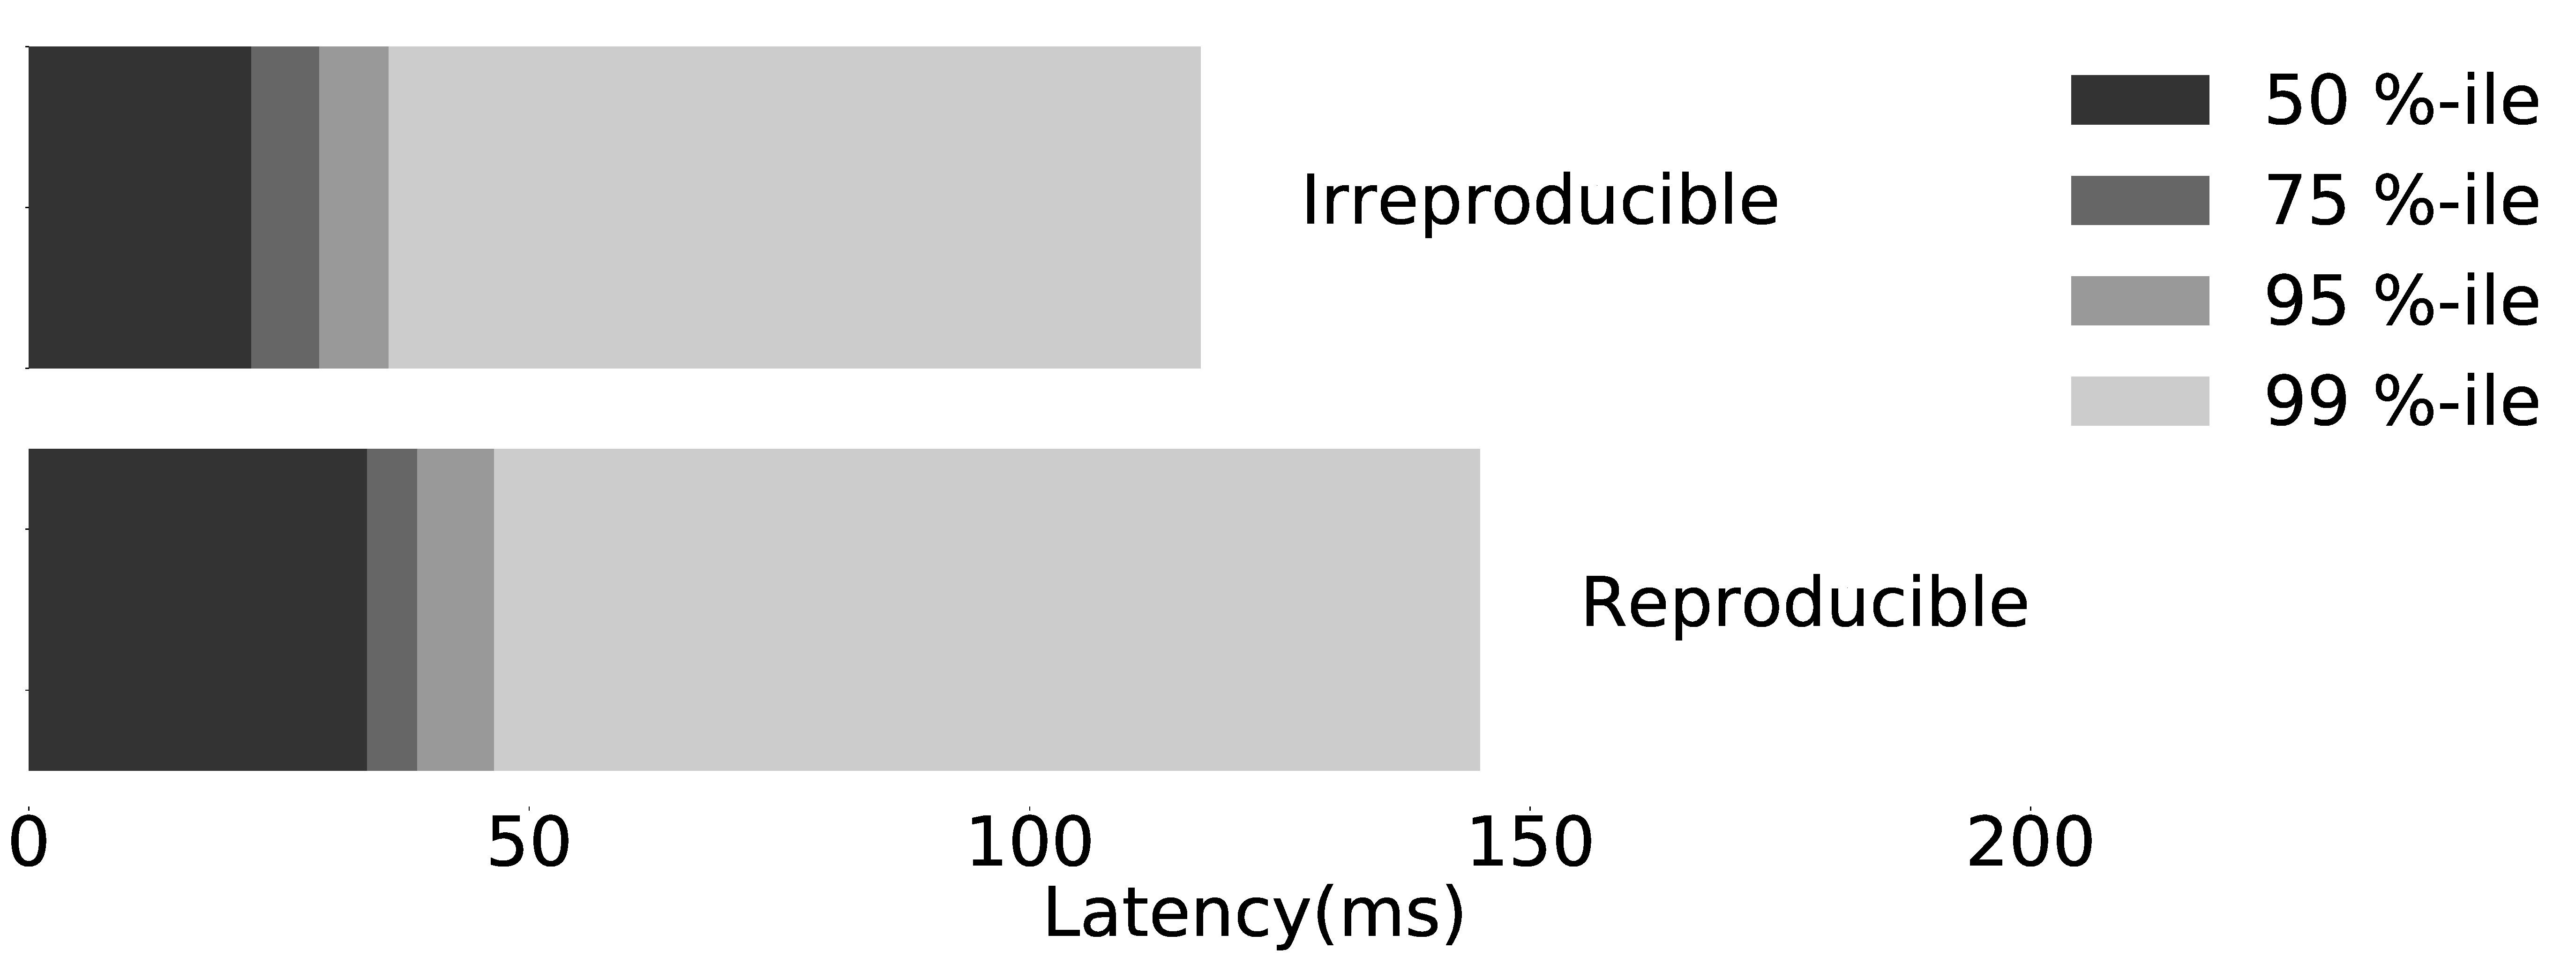
\includegraphics[scale=0.09]{pics/reproducibility}
  \caption{Latency comparison between reproducible and irreproducible data flows}
  \label {reproducibility}
\end{figure}

\subsection{Fault Tolerance}

As we demonstrated above, if machine learning pipeline is executed on multiple computational units, there can be issues with reproducibility. Unfortunately, it is not the only challenge: computational nodes and network failures may potentially cause shifted or even incorrect results. Despite the fact that failures are typically considered as edge cases, incorrect results obtained due to even rare instabilities may affect service reputation and lead to financial losses. Hence, in large-scale production deployments, it is important to ensure that nodes and network failures do not influence the outcome.

In stream processing systems, guarantees on data in case of failure are typically described in terms of {\em delivery guarantees}: at least once and exactly once. If a system provides exactly once, it is guaranteed that a streaming element is applied to data flow operators and released exactly one time. In other words, a system ensures that failure would be transparent for end-user. With at least once, it is ensured that an element is not lost, but it can influence operator states and be delivered to end-user multiple times. At least once may be preferred, because it typically has lower performance overhead. However, it is unclear in what degree such relaxation can influence the classification results. 

In order to demonstrate how the choice of a delivery guarantee affects text classification pipeline, we model two scenarios that can be faced, e.g. in news aggregators:
\begin{enumerate}
    \item There are two equally important events at the same time, e.g. football world cup and the G20 summit. Arriving news stories are grouped by these events: $n$ texts about football, then $n$ texts about politics and so on. This arrangement simulates articles from multiple sources. We expect that the proportion between the number of texts labeled as football and number of texts labeled as politics would be similar to the real distribution. Otherwise, news aggregator can make wrong conclusions about event importance and impact. The arose question is: can failure within at least once guarantee bias such distribution?
    \item Assume that news aggregator denotes topic as {\em popular} if the percent of articles labeled by this topic exceeds some threshold. For instance, in a day of Olympics opening ceremony, we expect that topic {\em sport} becomes popular as well as usual prevalent themes like politics or business. We simulate such a situation when some theme overcomes a given threshold under a normal execution or exactly once guarantee. Within the confines of this experiment, we aim to study if a failure under at least once guarantee can cause that the event does not exceed the threshold.    
\end{enumerate}

% In the following experiments, we demonstrate that at least once guarantee may not be acceptable in some cases. 

For the experiments, we set up 1 second between checkpoints in Flink, {\em RocksDB} as a state backend, and at least once as a delivery guarantee. It is worth to note that 1 second is the minimal snapshotting period that we were able to reproduce. The larger period can imply even more significant effects because in this case more elements are processed more than one time if a failure occurs.

\subsubsection{Biased results distribution}

In this experiment, we used a stream with 4000 articles. These articles can be considered as stories within a fixed time window and we are interested in the news topics distribution in this window. Articles are grouped in 4 blocks: 1st and 3rd contain news about football, and 2nd and 4th consisted of science news stories. We simulated a single node failure in both football and science groups. We denote that an article is classified into topic {\em Z} if it has the largest probability among all topics. Results are shown in Table~\ref{biased_results}. As one can notice, the classifier has an error: it labels approximately 42\% of articles as football and 40\% as science stories, while others are mistakenly classified as other topics. Nevertheless, it is important that results indicate a small difference between the number of football and news articles - about 1.5\%. The failure causes a significant shift of this distribution: as expected, a failure during football or science news implies repeated processing of the same articles. In both cases, there were repeated about 600 texts. As a result, we can see that the biased distribution, that is hardly similar to the original: the difference between the number of articles labeled as football and science becomes 7-10\%. 

\begin{table}[htbp]
\caption{Biased classification results due to failure within at least once guarantee}
\begin{threeparttable}
\begin{tabular}{lcl}
Experiment    & \% of football articles & \% of science articles    \\
\hline
Ground truth   &   50.0    &   50.0    \\
No failures*   &   41.8    &   40.4    \\
Failure on football**   &   46.7    &   35.5    \\
Failure on science**   &   37.7    &   44.5    \\
\end{tabular}
* or with enabled {\em exactly once} \\
** with enabled {\em at least once}
\end{threeparttable}
\label{biased_results}
\end{table}

\subsubsection{Invalid threshold}

% In the previous experiment, we demonstrated that failures can noticeably influence the distribution of classification results if there are few topics in an input stream. In this one, we show that the problem exists in a more general case. 

Test stream for this experiment contains 5000 articles. As in the previous experiment, we can denote them as news stories within a fixed time window. First 4450 articles in a stream have all possible 90 topics with the prevalence of football and politics. Last 550 texts consisted of news about animals. Such setup simulates some emerging event connected to animals. Assume that a news aggregator denotes topic as popular if it exceeds threshold 10\%. We simulated a single failure when the first 4450 articles were being processed.

Results of the experiments are shown in Table~\ref{biased_threshold}. It is expected that topic {\em animals} becomes popular. Without failures, this expectation is satisfied. However, failure with reprocessing of approximately 600 articles shifts the distribution of topics in results: the percent of articles labeled as animals story becomes 0.094. In this case, is not considered as popular and such behavior may affect news aggregation functionality.

\begin{table}[htbp]
\caption{Biased threshold due to failure within at least once guarantee}
\begin{threeparttable}
\begin{tabular}{lcl}
Experiment    & Top 3 topics    \\
\hline
Ground truth   &   Politics(11.5), Football(11.3),Animals(11.0)    \\
No failures*   &   Football(10.7),Animals(10.1),Politics(10.0)    \\
Failure**   &   Football(10.8),Politics(10.3),Animals({\bf 9.4})    \\
\end{tabular}
* or with enabled {\em exactly once} \\
** with enabled {\em at least once}
\end{threeparttable}
\label{biased_threshold}
\end{table}

\subsubsection{Overhead on exactly once}

In order to avoid results inconsistencies in case of failures, there is a need to enable exactly once delivery guarantee. Exactly once is implemented in Flink using a modification of the 2PC transactional protocol. A transaction starts when Flink injects a special element called {\em checkpoint} into the input stream. Each operation independently prepares data to save at the moment of checkpoint arrival. Prepared data is committed to external storage when checkpoint passes through the whole data flow. Output elements are released only after the transaction is committed. Because of the fact that a transaction begins once per snapshotting period, this period directly influences the latency of individual streaming elements.

Figure~\ref{fault_tolerance} shows latency comparison between runs within at least once and exactly once guarantees in Flink. As expected, latency in exactly once mode depends on the snapshotting period. Overhead on latency is significant even with 1 second between checkpoints: it is more than a second for all considered percentiles. Such behavior can be unacceptable in many real-life applications. Hence, there is a trade-off between latency of individual elements and a guarantee that failures do not affect classification results.

\begin{figure}[htbp]
  \centering
  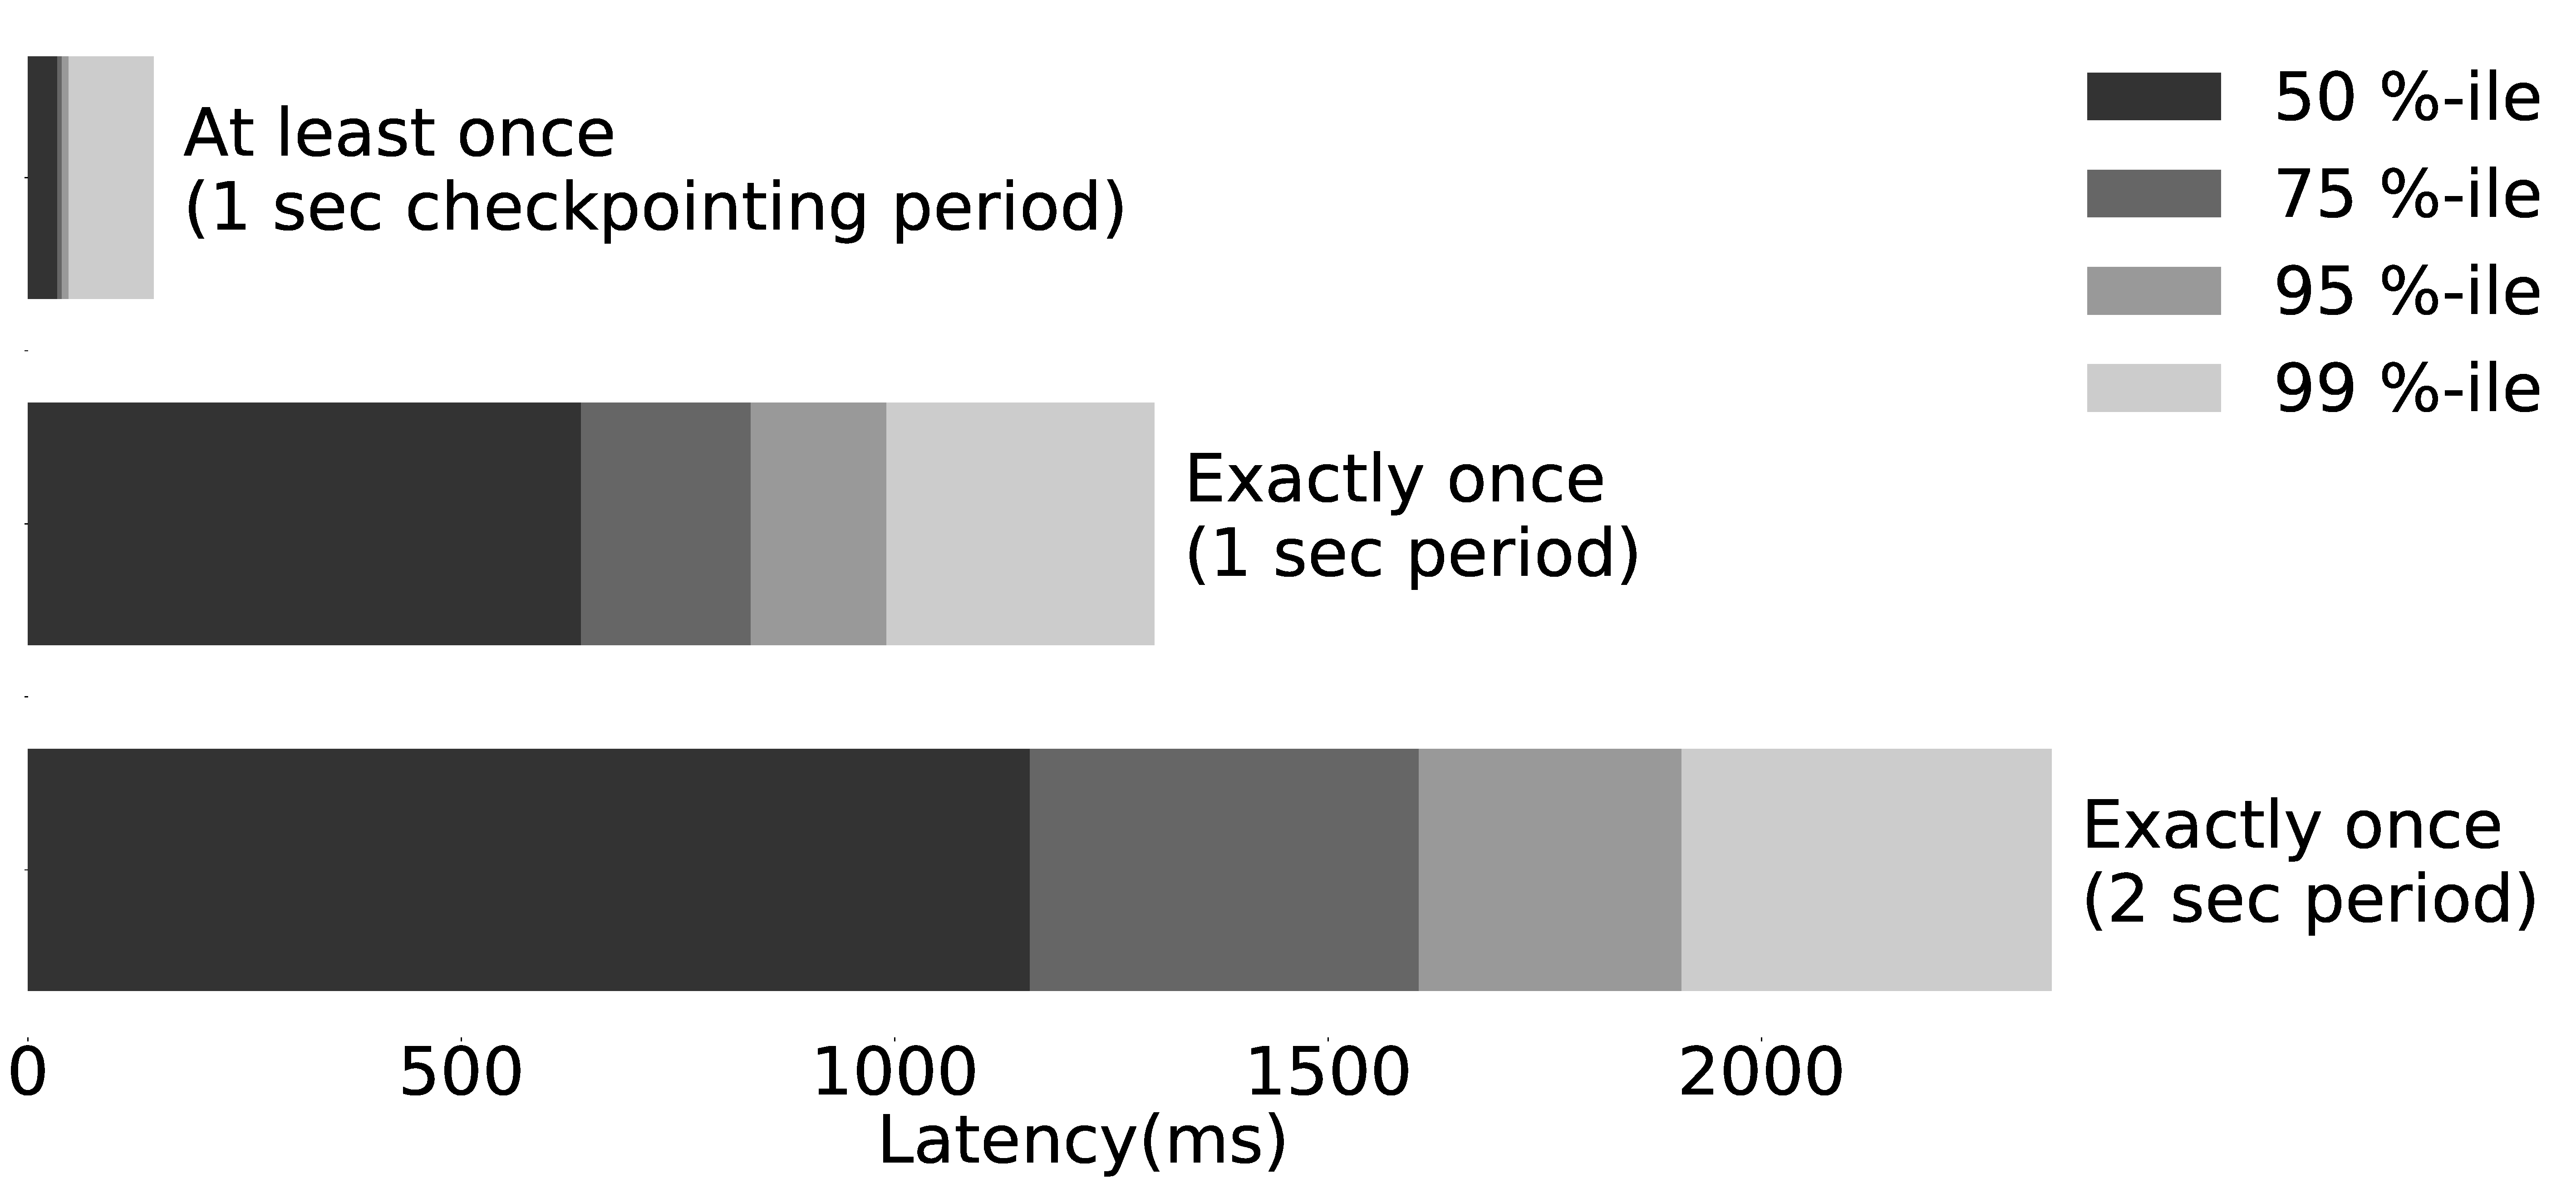
\includegraphics[scale=0.09]{pics/fault_tolerance}
  \caption{Latency overhead on exactly once}
  \label {fault_tolerance}
\end{figure}

